\documentclass{article}
\usepackage[utf8]{inputenc}

\usepackage{latexsym}
\usepackage{float}
\usepackage[utf8]{inputenc}
%\usepackage[catalan]{babel}
 \usepackage[english]{babel}
\usepackage{microtype}
\usepackage[hyphens]{url}
\usepackage{hyperref}
\usepackage{graphicx}
\usepackage{makeidx}
\usepackage{datetime}
\usepackage{multicol}
\usepackage{setspace}
\usepackage{enumerate}
\usepackage{booktabs}
\usepackage{listings}
\usepackage{color}
\usepackage{amsmath}
\usepackage{amssymb}
\usepackage[table,xcdraw]{xcolor}
\usepackage{graphicx}
\usepackage{listings}
\usepackage{hyperref}
\usepackage{vmargin}
\usepackage{wrapfig}
\usepackage{subfiles}
\usepackage{float}
\usepackage{amsmath}
\usepackage{amssymb}
\usepackage{tikz-cd}
\usepackage{multirow}
\usepackage{pgffor}
\usepackage{iflang}

%%%%%%%%%%%%%%%%%%%%%%%%%%%%%%%%%%%%%%%
%%%%%%%%%%%% UTIL COMMANDS %%%%%%%%%%%%  

\newcommand{\nc}{\newcommand}
\nc{\supindex}{\textsuperscript}

%%%%%%%%%%%%%%%%%%%%%%%%%%%%%%%%%%%%%%%
%%%%%%%%%%%%% CONFIG FILE %%%%%%%%%%%%%

\nc{\mytitle}{Multiple-choice online Exams}
\nc{\mysubtitle}{WS Project}
\nc{\authors}{Oriol Alàs Cercós, Marta Albets Mitjaneta}
\nc{\datetime}{11\supindex{th} of January, 2021}
\nc{\assignatura}{Distributed Computing}
\nc{\professorat}{Josep Lluís Lérida, Eloi Gabaldón, Jordi Gervàs}

% Per separar professors, utilitzar ','
% 	Ex: Maria, Joan, Pere

%%%%%%%%%%%%%%%%%%%%%%%%%%%%%%%%%%%%%%%
%%%%%%%%%%%%%  LANGUAGE   %%%%%%%%%%%%%

\newcommand{\tr}{\IfLanguageName{english}}

%%%%%%%%%%%%%%%%%%%%%%%%%%%%%%%%%%%%%%%
%%%%%%%%%%%%%%%%% MATH %%%%%%%%%%%%%%%%

\nc{\prob}[1]{P({#1})}
\nc{\probl}[2]{P({#1}|{#2})}

%%%%%%%%%%%%%%%%%%%%%%%%%%%%%%%%%%%%%%%
%%%%%%%%%%%%% TREE CREATOR %%%%%%%%%%%%

\setpapersize{A4}
\setmargins{2.5cm}  % margen izquierdo
{1.5cm}             % margen superior
{16.5cm}            % anchura del texto
{23.42cm}           % altura del texto
{10pt}              % altura de los encabezados
{1cm}               % espacio entre el texto y los encabezados
{0pt}               % altura del pie de página
{2cm}               % espaci\title{Determinització d'un autòmat finit}
\author{Oriol Alàs Cercós}
\date{29 d'Abril del 2019}

\def\contentsname{Índex}
\begin{document}
	

\begin{titlepage}
\begin{figure}[htb]
\begin{center}
	
\includegraphics[width=5cm]{imgs/UDL.png}
   	\vspace*{\stretch{1.0}}
   	\\
   	\medskip
   	\begin{center}
   		\noindent\rule{16.5cm}{0.4pt}
   		\medskip 
   		\\
      	\Huge\textbf{\mytitle}
      	\\\medskip 	\Large  \mysubtitle
      \\
      	
      	\noindent\rule{16.5cm}{0.4pt}
      	\\
      	\bigskip
      	\normalsize{\tr{Made by}{Realitzat per:}}
      	\\
      	\large\textit{\authors}
      	\\
      	\setlength{\parskip}{1em}
      	\normalsize{\tr{Delivery}{Data de lliurament:}}
      	\\
      	\large{\datetime}
   	\end{center}
   	\vspace*{\stretch{2.0}}
\end{center}
\end{figure}
\begin{flushright}
Universitat de Lleida
\\
Escola Politècnica Superior
\\
Grau en Enginyeria Informàtica
\\
\assignatura
\\
\medskip
\textbf{\tr{Professorate:}{Professorat:}}
\\
\foreach \n in \professorat{\n\\}
\end{flushright}
\thispagestyle{empty} 
\end{titlepage}
\tableofcontents
\thispagestyle{empty} 
%\newpage
\listoffigures
\listoftables
\thispagestyle{empty}
\newpage
\section{Introduction}
The actual project attempts to simulate a exams management application API. The used technologies in order to develop this project are:
\begin{itemize}
	\item \textbf{Dockerfile} and \textbf{Docker Compose} in order to have a virtual container of the project so as to deploy and run the application in different OS and machines without considering the terminal's specifications.
	\item \textbf{Django} web development framework with the \textbf{Rest API Framework} to make easy and more understandable the views and the development.
	\item \textbf{postgresql} database to store our data.
\end{itemize} 
\subsection{Usage}
If it is the first use of the project, you must build the images and create the container using:
\begin{verbatim}
	$ docker-compose build
\end{verbatim}
In order to run the container, you must use:
\begin{verbatim}
	$ docker-compose up
\end{verbatim}
You can run the container in a detach mode:
\begin{verbatim}
	$ docker-compose up -d
\end{verbatim}
If you want to build and run the container in a same command, you can also use:
\begin{verbatim}
	$ docker-compose up --build
\end{verbatim}
When it is up, it is required to build the database stored in \texttt{./database/data/}, using in the root directory:
\begin{verbatim}
	$ docker-compose exec web python manage.py migrate
\end{verbatim}
This command will translate the \texttt{exams/models.py} into a \textit{postgresql} data and it will store the tables in \texttt{./database/data/}.
\\
\\
As it has been created tests, the way to run them all is:
\begin{verbatim}
$ docker-compose exec web python manage.py test apps.api.tests.AllInOneTestCase
\end{verbatim}
It has been created an only test case class because that by creating more than one, the unit tests may fail because of database concurrency (e.g, creating an exam in one use case and proving that there are no exams in another case).
\section{Django}
Django is a high-level python web framework that encourages rapid development and clean, pragmatic design, based on MVC. Despite that fact, it uses Model-View-Template design.
\begin{itemize}
	\item Model or data representation. It defines the structure of the store data in our database.
	\item View or business logic representation.
	\item Template or user-centered representation. Designer plain-text system where the views are displayed.
\end{itemize}
Moreover, Django is a loosely coupled framework that can have several features in different packages called \textit{applications}. Django app is a self-contained package. That's why in our apps directory, it appears two applications called:
\begin{itemize}
	\item Exams. Application where contains the data representation of the our models.
	\item API. Application where contains the logic of our project. As it uses MVT design, the models are imported from exams application to create the views. The template part is implemented by the \textit{Django Rest Framework}. Even though, it is required to have a serializer class to transform the models objects of our database to rest objects\footnote{Using JSON format.}.
\end{itemize}
Also, Django has already an admin administration to view all the data in a way not depending on the API. The endpoint to go the administration system is \texttt{/admin/}. Also, it is required to create a super user to authenticate as admin user.
\begin{verbatim}
$ docker-compose exec web python manage.py createsuperuser
\end{verbatim}
\section{Classes}
\begin{figure}[H]
	\centering
	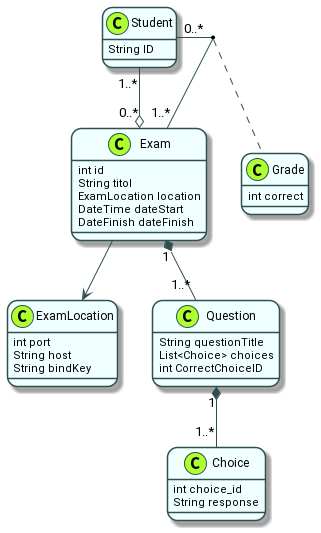
\includegraphics[width=7cm]{imgs/models.png}
\end{figure}
The classes for our database represented in \texttt{exams/models.py}.
\begin{itemize}
	\item \textbf{Student}. This class will be used to keep the students’ id that will be necessary when we want to know if a student is allowed or not to take an exam. For now, it is only required to have the ID of the student.
	\item \textbf{Exam}. As the name says, it is the exam information. It is our main class as it is connected with all of the others. In addition of having its title, description and other value fields, this model has the needed foreign keys to relate with the other models.
	\item \textbf{Exam Location}. It contains the host, port and the binding key of the RMI project in order to connect to the RMI server.
	\item \textbf{Question}. It contains the data representation of a question with its answers and the index of the correct one.
	\item \textbf{Choice}. Data representation of an answer.
	\item \textbf{Grade}. Data representation of a student's grade of an exam.
\end{itemize}
\section{Endpoints}
The most important endpoints for this project are in \texttt{api/urls.py}. The presentation of the endpoints can be found in the slides presentation with the screenshots of each case execution.
\\
\\
The real schema of the endpoints can be seen also in \texttt{/api/schema/}.
\section{Integration with the RMI Assignment}
In order to develop the features described in the assignment documentation, it has been created a package to create the interaction with the API. This package allows a loosely coupled implementation with the minimum changes of the responsibilities of the classes already implemented.
\\\\
\textbf{MyExams }class will use the HttpRequest and the HttpClient classes to interact with our API. As we are developing a REST API, our methods can be static as it is stateless.
\\\\
After implementing our API adapter for our Java project, our RMI system design must change. While the server must import the exam data from a source and make a post request to the API to store the exam information to the WS, the client part must verify that the studentID is on the list of the current exam. As our client does not know the ID of the exam, it has been relaxed the situation and the professor will show the id of the exam and the client program must put this id as an argument.
\\
\\
After finishing the exam, the server must save the grades and store them in the WS.
\subsection{Technologies implied}
Within the new requirements, our RMI project must load and serialize JSON objects to Java objects. To do that, it is used a maven repository called \texttt{com.fasterxml.jackson}.
\\
\\
It is also used \texttt{java.net} to interact with the WS.
\section{Conclusion}
Also, our API contains a documentation system where explains how to use our application and an interact mode in \texttt{/api/docs/} and a schema in \texttt{/api/docs/}.\\\\
The time estimated of the work is about 100 hours more or less, as we are 2 members and we have worked 50 hours each one.\\\\
Our API can be found in \url{https://github.com/Oriolac/my-exams-api}. Our RMI Project can be found in \url{https://github.com/Marta99/multiple-choice-exam/}.
\end{document}
